\section{\ball -  \ballFull}
\label{sec:ball}
As already mentioned, the main intention for the development of \ball as well as for \biochem is to generate a framework for rapid prototyping of molecular applications. This section summarizes the key concepts of \ball that motivated the design of our project \footnote{An in-depth description of the entire \ball framwork is beyond the scope of this article. Confer the main publications~\cite{kohlbacher_ballrapid_2000, hildebrandt_ball_2010}  for more details.}\\
The initial work on the \ball project started in 1996, resulting in the C++-written library \ball and its accompanying molecular viewer, \textit{\ballview}. One reason for the success of \ball is its sophisticated design; it is an  object-oriented project with four design goals as shown in Table~\ref{table1_design_goals}.

\begin{table}

	\tbl{Desing goals of \ball}{
		\begin{tabular}{|c|c|}\hline
		
		Ease of use &  Robustness \\\hline
		Openness  & Functionality \\\hline
	\end{tabular}}
	\label{table1_design_goals}
\end{table}

The object-oriented approach facilitates ease of use in combination with the well documented and intuitive interface. As can be seen in Figure~\ref{fig:ball_architecture} \ball is structured in several layers. On top of the standard template library (STL), resides the foundation classes, providing a set of general data structures such as hash sets and mathematical objects (e.g. matrices, vectors,...). The third layer is the actual core of the library: the \texttt{KERNEL} classes, which contain data structures for molecular entities. The basic components represent fundamental functionalities and are placed on top of the core, with the exception of the visualization module that is based on QT and Open GL \cite{qt,OpenGLWebsite} . Finally, the application layers can be used to develop own applications or use the available tools. \\
Hildebrandt et al. published an updated version in 2010, featuring the CMake-Buildsystem and Python bindings. These additions improved usability and openness, allowing easier integration of external packages and increased portability to other compilers and operating systems. \\

\ball's uniqueness stems from its rich functionality integrated in a single easily extensible open-source platform. Figure~\ref{fig:ball_structure} shows the kernel and its classes are forming three different frameworks: the general molecular framework, the protein and the nucleic acid frameworks. All kernel classes are implemented through the realization of a composite pattern. More precisely, the composite class is the base class for all derived classes representing molecular entities such as \texttt{Atom}, \texttt{Protein}, etc. or container classes \texttt{System}, \texttt{AtomContainer}, and so on. 
Based on these three frameworks, \ball provides functionalities for various different steps in molecular analysis ranging from tools for preprocessing such as file import and export, addition of missing atoms, normalizing name schemes, to complex molecular structure analysis (energy minimization, mapping) and advanced solvation methods. These implemented applications are well-tested and validated, ensuring robustness.  \\
\ball's well-designed and structured nature has contributed to its long-lasting popularity, with one of the largest user communities for open-source software in its field.



\begin{figure*}[t]
	\centerline{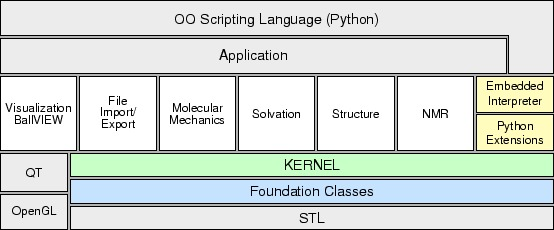
\includegraphics[width=11cm]{gfx/BALL-architecture.jpeg}}
	\caption{\ball's architecture is structured in several layers. Upon the standard libary layer are the foundation classes and ontop of them the kernel. Several module extend the interface for visualization, file import and expoert, molecular mechanics, solvation, structure and NMR. The C++ written frameworkis extended by Python interface for fast scripting purposes. The figure was taken from the official \ball documentation \cite{BALLTutorial}.}
	\label{fig:ball_architecture}
\end{figure*}



\begin{figure*}[t]
	\centerline{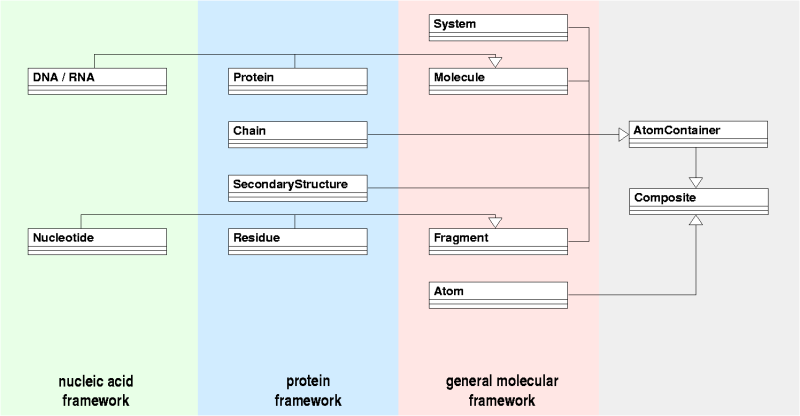
\includegraphics[width=14cm]{gfx/KERNEL.png}}
	\caption{UML class diagram of the kernel classes. The kernel classes form three frameworks and are implemented using the composite pattern. The figure was taken from the official \ball documentation \cite{ball_tutorial}.}
	\label{fig:ball_structure}
\end{figure*}
